\section{Adaptive Music System}
\label{sec:ams}

In the year 2019, the authors Patrick Hutchings and Jon McCormack
introduced the Adaptive Music System (AMS) \cite{hutMcCormAms} 
and tested it with several evaluators. It was developed as a
stand-alone package that receives game information from the
video game itself in real-time to generate a model of the game-
state and output music from this state \cite{hutMcCormAms}.
Their system is divided into two main components: 
\begin{enumerate}[label=\arabic*)]
    \item A spreading activation model to read the game's information by
analyzing the emotion the player might feel currently\cite{hutMcCormAms}.
    \item The music generation system that uses the spreading activation model output to generate its music \cite{hutMcCormAms}. 
\end{enumerate}
\begin{figure}[h]
    \centering
    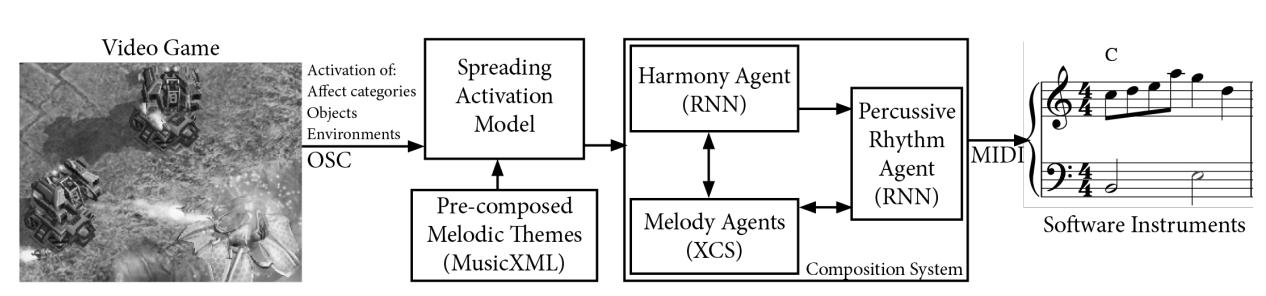
\includegraphics[width=\linewidth]{images/ams_architecture.png}
    \caption{Architecure of AMS \cite{hutMcCormAms}}
    \label{fig:ams_architecture}
\end{figure}
A first introduction of the system can be seen in \Cref{fig:ams_architecture}.
It represents the whole workflow of music generation \cite{hutMcCormAms}. The game 
acts here as an input for the Spreading Activation Model, which passes its output
to the music Composition System \cite{hutMcCormAms}. The composition system itself consists 
of three types of components: a harmony agent, several melody agents (one per instrument)
and a percussive rhythm agent. The system outputs music in
MIDI format \cite{hutMcCormAms}. MIDI (Musical Instrument Digital Interface) is a
common music format \cite{midi_explanation} that can also be used as a protocol
between computers and synthesizers \cite{midi_explanation}. It can be also used to 
generate synthesized music \cite{midi_explanation} with many types of instruments \cite{midi_general}.
The MIDI files are then used to generate Music with specific software systems \cite{hutMcCormAms}. MIDI uses hexadecimal values in order
to represent the volume, pitch, instrument etc. \cite{midi_general}\cite{midi_explanation}.

\subsection{Spreading Activation Model}

The spreading activation model \cite{collins1975spreading} itself is a knowledge 
organisation model, which can be used to understand and capture emotion \cite{hutMcCormAms}\cite{carr1982words} in a graph, making it 
worth being used in a video game \cite{hutMcCormAms}.

For the AMS, the authors described the implementation
of the spreading activation model as a weighted and 
undirected graph \( G = (V, E) \)\cite{hutMcCormAms}, where 
\( V \) represents the vertices, and \( E \) the edges of the
graph. Each node \( V \) of the graph 
stands for a certain context \cite{hutMcCormAms}, which can
be either an affect \( (A) \), an  \( (O) \) object or an environment \( (N) \) \cite{hutMcCormAms}. A node
contains an activation value from 0 to 100 \cite{hutMcCormAms}. The 
edges of the graph stand for the level of  association 
of those context objects \cite{hutMcCormAms} 
and have normalised weights \( w_E\). Nevertheless, the authors
say that the nodes do not have to be connected, and edges do not 
form between affects \cite{hutMcCormAms}. 

Initially at the game
start, the graph contains the affect nodes sadness, happiness, 
threat, anger, tenderness and excitement \cite{hutMcCormAms}
and receives updates from the game every 30ms \cite{hutMcCormAms}.
The model uses an Open Sound Control (OSC) client to refresh
the graph with the game information, and nodes are newly generated
when a concept is not contained within the graph.

Nodes which contain a positive activation level are able to activate
adjacent nodes \cite{hutMcCormAms}. The activation done proportionally to the weights
of the edges \cite{hutMcCormAms}. For instance, if a Node A has an activation level
of 50 and has an adjacent node B, connected with an edge weight
of 0.25, Node A will activate Node B with at least 12.5 \cite{hutMcCormAms}. If
the Node has already been activated with the same or a higher
value, the vertex weight stays the same. The activation
can be described as \[
w_B := 
\begin{cases} 
w_A * w_E & \text{if } w_A * w_E > w_B \\
w_B & \text{if not} 
\end{cases}
\] 
where \( w_A \) is the activation value of vertex A, \( w_B \)
is the activation of vertex \(B\) and \( w_E \) is the normalised value
of the edge connecting both vertices together \cite{hutMcCormAms}.

Both the activations of nodes and the weights of edges diminish
over time \cite{hutMcCormAms}. In the tested game scenarios, 
explicitly defined associations do not fade, while inferred 
associations decay at a rate of 0.01 per second and node 
activations decrease at a rate of 0.1 per second
\cite{hutMcCormAms}.
Melodic themes have been precomposed for well-known objects and are implemented as properties of object nodes within the system \cite{hutMcCormAms}. The music composition system continuously generates new music based on the knowledge contained in the graph to accompany gameplay \cite{hutMcCormAms}. 

\subsection{Music Composition System}

\begin{figure}[h]
    \centering
    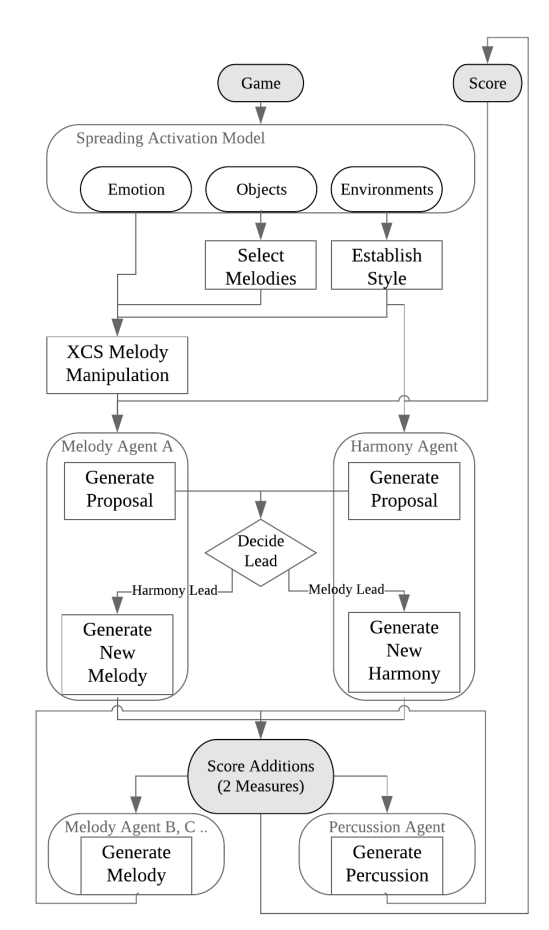
\includegraphics[height=9cm]{images/ams_system_diagram.png}
    \caption{System diagram of AMS \cite{hutMcCormAms}}
    \label{fig:ams_system_diagram}
\end{figure}

The authors designed their system to be a multi-agent composition system \cite{hutMcCormAms} and it is based on group dynamics of 
improvising musicians and different algorithmic composition
techniques \cite{hutMcCormAms}.
They also describe the co-agency of the system, where all agents
of the system work towards the same goal: generating music, like
real musicians would do \cite{hutMcCormAms}.
In the AMS of the authors, they implemented three different agents:
an harmony agent, melody agents and a percussive rhythm-agent \cite{hutMcCormAms}.

\subsubsection{Harmony Agent}

The harmony agent is implemented as a Recurrent Neural 
Network (RNN) using Gated Recurrent Units and two hidden
layers with 192 units each \cite{hutMcCormAms}.
It was trained with chord symbols from 1800 songs from
the Nottingham Music Database, 2000 songs from the
Wikifonia Database in the genres rock, pop and 2986 jazz songs \cite{hutMcCormAms}.
For the training itself, they were using style tokens
like pop, rock, jazz and folk and used dynamic unrolling 
for a faster training time using 100 dimension encoding stated to be the most performant variant tried by the authors \cite{hutMcCormAms}.
The last layer of the neural network uses a softmax
activation layer, which gives probabilities for the 
next following chords \cite{hutMcCormAms}. The generated chord is put into a chord progression
for the composition and put those generated chords back
into the the agent to progress the further generation 
of chords \cite{hutMcCormAms}. They also describe that
the softmax layer output serves as a confidence score.
This confidence score is used to be compared with other
agents \cite{hutMcCormAms}. If the confidence score of
the harmony agent is higher than the one of the first
melody agent, the harmony agent is activated 
and searches for a suitable harmonical melody 
\cite{hutMcCormAms}. They also explain that the harmony
agent itself does not generate any notes, but produces a
harmonic context that is used by the melody agents
in order to write phrases for the instruments \cite{hutMcCormAms}. This described context is designed
as a 2D matrix, which can be seen in \cite{hutMcCormAms}.
The matrix as described by the authors Hutchings and 
McCormack shows which tones most strongly indicate a chord
of a musical measure \cite{hutMcCormAms}.

\subsubsection{Melody Agents}

The melody agents (one per instrument) are responsible
for the generation of melodies in a computer game, based 
on the emotions, objects and environments in the graph
resulting from the spreading activation model \cite{hutMcCormAms}, adding melodies every two measures \cite{hutMcCormAms}.
The authors used an eXtended Classifier System (XCS) in
order to develop rules for precomposed melody fragments \cite{hutMcCormAms}.
Those melody fragments, which were composed by from 
experts from different concerts, have a length of one to 
four measures and are edited with eight melody operators
like reversing, shortening, lengthening and inverting, and 
also combinations of all four of them \cite{hutMcCormAms}.

All melody agents work every two measures, whereas the
first melody has the highest pitch, and the second melody 
has the lowest pitch \cite{hutMcCormAms}. The authors conclude that the 
maximum sound range is dependent of the number of agents
and the music style \cite{hutMcCormAms}.
The harmony agent generates accords based on styles like
jazz, folk, rock and pop while the melody agents 
have the responsibility to evaluate those proposals \cite{hutMcCormAms}.

\subsubsection{Percussive Rhythm Agent}

The percussive rhythm agent is also based on a RNN and
has the responsibility to add a rhytmic component to
the created piece \cite{hutMcCormAms}.



The whole flow of the music generation of AMS can be seen in 
\Cref{fig:ams_system_diagram}. The spreading activation model creates a graph
and passes it to the composition system itself and selects pre-defined melodies
and style \cite{hutMcCormAms}. Those get passed to the melody agents and the harmony agents \cite{hutMcCormAms}.
The confidence scores of the first melody agent and the harmony agent are compared
with each other in order to determine which proposal will be generated \cite{hutMcCormAms}.
After the generation process, the percussive rhythm adds a rhythmic component if needed \cite{hutMcCormAms}.






